\chapter{I Asked Texan Millionaires Their Best Financial Decision}

This chapter is built from an interview montage rather than from a blackboard derivation, and that changes the character of the notes. We do not have visible board mathematics to transcribe. Instead, we take the spoken claims seriously and compress their mechanisms into a small amount of editorial mathematics whenever that helps. The lecture opens with the hardest question in the simplest language: how does one become financially free in today's world? The first answer already places a constraint on the whole discussion: it takes time. From there the argument accumulates through cases---early asset selection, savings discipline, the value of one's own contribution, the bottlenecks of scale, passive income, slow investing, risk, and finally the social temperament of wealth.

\section{Opening Question: Freedom and the First Constraint of Time}

The cold open gives us the governing problem before anything else: what would it mean to be financially free, not merely employed at a high salary, but genuinely rich? The answer that comes back is almost austere in its simplicity: it takes time. We should keep that opening discipline. The lecture does not begin with tricks, hacks, or exotic instruments. It begins by refusing immediacy.

\begin{definition}[Operational criterion of financial freedom]
A compact way to summarize the lecture's central criterion is
\begin{equation}
C_{\text{passive}} \ge E_{\text{life}},
\end{equation}
where $C_{\text{passive}}$ is the cash flow arriving without continuous labor, and $E_{\text{life}}$ is the stream of recurring living expenses.
\end{definition}

\begin{remark}
No speaker writes this inequality on a board; it is an editorial compression of the lecture's most explicit answer later in the video. But it captures the structure faithfully: freedom is not defined by prestige alone, but by the separation of income from immediate labor.
\end{remark}

The host introduction in downtown Austin then reframes the lecture as field inquiry. We will not be told one theory from one speaker. We will move from person to person and let the mechanism of wealth reveal itself piece by piece.

\section{Early Accumulation: Assets, Savings, and Diversification}

\paragraph{Anecdote.}
The first interviewee gives the classic asset-side answer: the best financial decision was to invest early in IT stocks, specifically Intel and Microsoft, with Microsoft held for more than twenty years. This is followed, almost immediately, by advice to a younger self: save money, invest, do not spend more than you have, maintain a diverse portfolio, and leave the 401(k) alone.

\paragraph{Claim.}
The lecture begins by insisting that wealth can start from patient ownership of productive assets, but only if income is not consumed as fast as it is earned.

\paragraph{Mechanism.}
If we let $Y$ denote earned income, $C$ consumption, and $S$ retained savings, then the transcript's discipline may be written as
\begin{equation}
S = Y - C, \qquad C \le Y.
\end{equation}
The second inequality is simply the spoken prohibition against spending beyond one's means.

A minimal notation for diversification is
\begin{equation}
D=\{a_i\}_{i=1}^{n}, \qquad n \ge 2,
\end{equation}
where the point is not to formalize modern portfolio theory in full, but to preserve the lecture's plain insistence that one should not hang everything on a single asset.

\subsection{A Worked Accumulation Rule}

Once we have savings, the lecture's slow machinery becomes clear. One buys productive assets early, continues to add capital, and then lets time do work. A compact update rule is
\begin{equation}
W_{t+1}=(1+r)W_t+s_t,
\end{equation}
where $W_t$ is net worth at time $t$, $r$ is a long-run return on the existing asset base, and $s_t$ is the investable surplus contributed during period $t$.

Iterating once or twice shows the structure:
\begin{align}
W_1 &= (1+r)W_0+s_0,\\
W_2 &= (1+r)W_1+s_1 \\
    &= (1+r)^2 W_0 + (1+r)s_0 + s_1.
\end{align}
Proceeding in the same way, we obtain the closed form
\begin{equation}
W_t = W_0(1+r)^t + \sum_{k=0}^{t-1} s_k(1+r)^{\,t-1-k}.
\end{equation}

This is not spoken in symbolic form, but it is exactly the content of the early interview cluster. The Microsoft position held for ``20 plus'' years is the long horizon; the injunction to save and keep investing supplies the recurring $s_k$; diversification keeps the whole process from collapsing into a single speculative bet.

\section{Value Creation as Career Capital}

The lecture then pivots. We move from buying the right assets to refusing the wrong price for one's own contribution. One interviewee says that the best financial decision she ever made was to walk away when someone did not value what she brought. The impact, she says, was enormous: the next opportunity confirmed that the value was indeed there.

\paragraph{Anecdote.}
This is not portfolio selection in the narrow sense. It is a pricing decision about the self.

\paragraph{Claim.}
For entrepreneurs and operators, the person may be part of the asset base. In that case, wealth does not come only from appreciation in market instruments; it also comes from how correctly one prices and captures one's role in value creation.

\paragraph{Mechanism.}
A useful accounting identity is
\begin{equation}
\Delta W = S + \Delta A + \Delta B - C_{\text{excess}},
\end{equation}
where $\Delta A$ is appreciation in financial or real assets, and $\Delta B$ is the increase in business equity, ownership, or operator-linked value capture. The point of the interview is that a person who remains systematically undervalued suppresses $\Delta B$.

We may summarize the lecture's implicit operator logic by the schematic relation
\begin{equation}
\mathcal{O} \longrightarrow \text{value creation} \longrightarrow \text{bargaining power} \longrightarrow \text{ownership or compensation}.
\end{equation}
Again, the notation is ours, but the sequence is the speaker's: when the entrepreneur is ``the value creation,'' wealth depends not only on effort, but on how much of the created value is retained.

\section{Scaling a Business: Leverage, Money, Cash Flow, Delivery}

We now shift from personal valuation to business architecture. The CEO interview asks what it takes to move a business from six to eight to ten figures, and the answer is remarkably concrete. One needs leverage. One needs the money to get there. Cash flow is king. And one must actually be able to deliver the service line. Only then can one move through the plateau and into the next ``hockey stick.''

A compact way to formalize that advice is
\begin{equation}
F_{\text{scale}} = \min\{L,M,CF,Q\},
\end{equation}
where $L$ is leverage, $M$ available money or capital, $CF$ cash flow, and $Q$ delivery capacity. The minimum governs the rate at which scale is possible. If one term is weak, the system stalls there.

This is a good example of how the lecture introduces a new mathematical move. It does not begin with abstraction. It begins with a practical question about scaling. Only after the pressure point is named do the operative constraints appear. The lesson for the notes is that we should not present these four objects as a generic business checklist. They arise because the lecture wants to know why some firms remain trapped on a plateau while others can actually climb.

The startup advice that follows belongs here as well. ``You don't know everything.'' Seek advice. Do not try to be everything for everybody. Have a unique idea. Back yourself, or find people who believe in it, or get a partner. All of this is the human corollary of the bottleneck equation: if scale depends on several constrained variables, self-sufficiency is rarely the right description of the process.

\section{Passive Income and Capital Allocation}

The lecture reaches its central payoff in the interview with the founder who says the best financial decision was simply working for himself. He reports building a company, selling it at age thirty-three, retiring, and then returning to work. The transcript gives the sale amount in unstable form as ``1 billion, 30 million,'' and the exact number should be treated cautiously. What matters most here is not the precise normalization of the exit, but the way the story resolves the chapter's opening question.

\subsection{Question \& Answer}

\paragraph{Question.}
How can someone become financially free in today's world?

\paragraph{Answer.}
By finding or building something that creates revenue when one is not physically working: investments, owned property producing rent, inventions, products, or businesses whose cash flow is not tied hour by hour to the owner's labor. This is the lecture's clearest answer, and it is why the opening inequality is not merely decorative.

The lecture immediately turns that answer into a capital-allocation question: once money begins to accumulate, where should it go? The answer is not singular. Long-term real estate is described as a ``consistent good play,'' while technology stocks and the stock market remain viable channels as well. The important thing is that allocation is asked only after the revenue-without-labor mechanism is stated. The order matters.

\begin{figure}
\centering
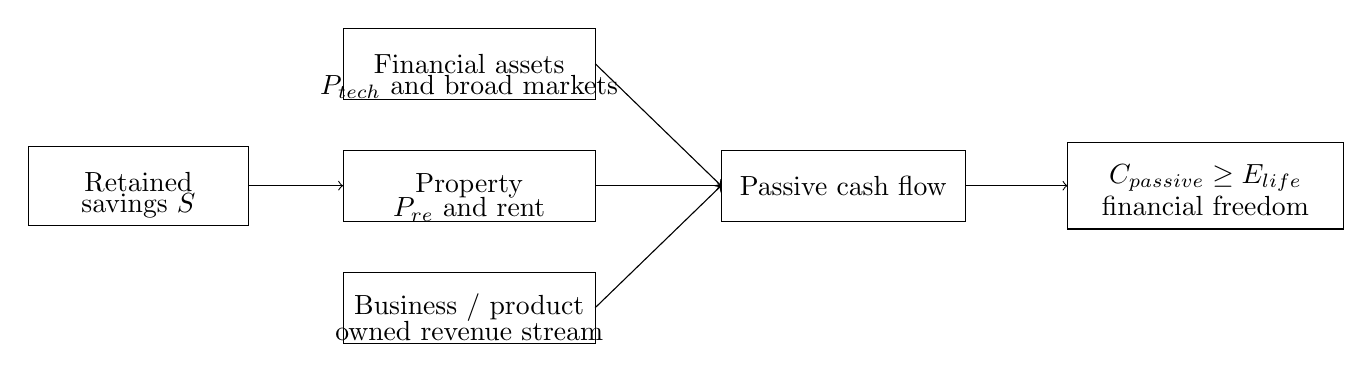
\begin{tikzpicture}[x=1cm,y=1cm]
\draw (0,2.6) rectangle (2.8,3.6);
\node at (1.4,3.15) {Retained};
\node at (1.4,2.85) {savings $S$};

\draw[->] (2.8,3.1) -- (4.0,3.1);

\draw (4.0,4.2) rectangle (7.2,5.1);
\node at (5.6,4.65) {Financial assets};
\node at (5.6,4.35) {$P_{\text{tech}}$ and broad markets};

\draw (4.0,2.65) rectangle (7.2,3.55);
\node at (5.6,3.10) {Property};
\node at (5.6,2.80) {$P_{\text{re}}$ and rent};

\draw (4.0,1.1) rectangle (7.2,2.0);
\node at (5.6,1.55) {Business / product};
\node at (5.6,1.25) {owned revenue stream};

\draw[->] (7.2,4.65) -- (8.8,3.1);
\draw[->] (7.2,3.10) -- (8.8,3.1);
\draw[->] (7.2,1.55) -- (8.8,3.1);

\draw (8.8,2.65) rectangle (11.9,3.55);
\node at (10.35,3.10) {Passive cash flow};

\draw[->] (11.9,3.1) -- (13.2,3.1);

\draw (13.2,2.55) rectangle (16.7,3.65);
\node at (14.95,3.20) {$C_{\text{passive}} \ge E_{\text{life}}$};
\node at (14.95,2.85) {financial freedom};
\end{tikzpicture}
\end{figure}

This diagram is an editorial reconstruction, but it is faithful to the transcript's order: first retain earnings, then acquire productive claims, then let those claims feed a cash-flow stream that can eventually cover life itself.

\section{Slow Investing, Bubble Risk, and the Difference Between Gambling and Investing}

The lecture now inserts a cautionary counterweight. Another interviewee says the best financial decision was entering a profession with job security, never living beyond one's means, and making sensible investments. Asked for advice on investing, he says to study the subject, not to do what the herd is doing, and to distinguish sharply between investment and gambling.

We should preserve that distinction explicitly:
\begin{equation}
\text{Investing} \neq \text{gambling}.
\end{equation}

The lecture then gives a specific example of how this distinction behaves in practice. Even a strong local market such as Austin real estate can show bubble tendencies. Thus, ``real estate'' is not an unconditional command. A good asset class does not abolish timing risk. The recommendation becomes more nuanced: slow and steady, studied entry, and suspicion of crowd frenzy.

In the language of the earlier equations, this section warns us not to misread $r$ as an entitlement. The accumulation rule is not a promise that every popular asset deserves capital. It is a description of what happens when sound surplus is placed into productive claims and held with discipline.

\section{A Harder Landscape: Competition, Risk, and the Entrepreneurial Temperament}

At this point the lecture broadens its field of view. Financial freedom, one speaker says, is getting harder. Competition is now global. One is not merely competing locally, but against people willing to work with extreme intensity. The phrase about sleeping four hours a night is not a model, but it is a statement about the supply side of ambition in the present market.

The hosts then pivot into interpretation. Austin, they suggest, can hide enormous wealth beneath ordinary clothing and ordinary street presence; Dallas is described as more visibly status-oriented. This digression is not accidental. It helps explain why several of the earlier interviewees sound almost anti-flashy. Wealth, in this lecture, is repeatedly attached to process rather than display.

\paragraph{Anecdote.}
A later interviewee says he bought property in Bee Caves twenty-five years ago, and it became very valuable. Asked again how one becomes financially free, he repeats the opening lesson: it takes time. Asked what enabled his success, he answers: he took chances.

\paragraph{Claim.}
Time and risk are not competing principles. They are complementary ones. Time governs compounding; risk opens the door to large gains that would otherwise never exist.

\paragraph{Mechanism.}
The lecture supports only a weak necessary statement,
\begin{equation}
\text{Risk} > 0,
\end{equation}
not as a portfolio-optimization theorem, but as a refusal of perfect safety as a route to substantial wealth. No one here offers a formal risk-return frontier. The point is more basic: without exposure, nothing large can be built or acquired.

This section also gathers the lecture's social mechanism of entrepreneurship. Entrepreneurs respect hustle because they remember having to ask for meetings, contacts, collaborations, and chances. They light up, the hosts say, before one even knows what they own. The closing examples reinforce the same pattern: learn from people who know what they are doing, make good connections, buy productive property early when one can, find advice that fits one's own situation, and take more risks while worrying less about immediate judgment.

\section{Summary}

The lecture begins by denying instant wealth and ends by explaining why that denial is useful. Financial freedom is not introduced as glamour but as a structure: earn, retain, invest, own productive claims, let time work, and aim for income that survives the interruption of labor. Along the way the interviewees add the missing corrections. One must not overspend. One should diversify. One's own contribution may itself be a source of value capture. Scale is bottlenecked by leverage, money, cash flow, and delivery. Slow investing is different from gambling. Good assets can still be mistimed. And wealth, if it becomes durable, requires not only patience but also risk, judgment, and the willingness to keep building long after the quick answer would have been more emotionally satisfying.